\documentclass{thesis-library}

\usepackage{lipsum}
\usepackage{booktabs}
\usepackage{multirow}
\usepackage{array}
\usepackage{amsmath}
\usepackage{amssymb}
\usepackage{hyperref}
\usepackage{xcolor}
\usepackage{listings}
\usepackage{caption}
\usepackage{subcaption}
\usepackage[utf8]{inputenc}
\usepackage{float}

% -------------------------------------------------------
% Acronyms / Abbreviations
% -------------------------------------------------------
\newacronym{just}{JUST}{Jashore University of Science and Technology}
\newacronym{cse}{CSE}{Computer Science and Engineering}
\newacronym{ev}{EV}{Electric Vehicle}
\newacronym{soc}{SOC}{State of Charge}
\newacronym{sumo}{SUMO}{Simulation of Urban Mobility}
\newacronym{traci}{TraCI}{Traffic Control Interface}
\newacronym{ml}{ML}{Machine Learning}
\newacronym{rf}{RF}{Random Forest}
\newacronym{dt}{DT}{Decision Tree}
\newacronym{lr}{LR}{Linear Regression}
\newacronym{xgb}{XGB}{Extreme Gradient Boosting}
\newacronym{rmse}{RMSE}{Root Mean Square Error}
\newacronym{mae}{MAE}{Mean Absolute Error}
\newacronym{r2}{R\textsuperscript{2}}{Coefficient of Determination}
\newacronym{fifo}{FIFO}{First In First Out}
\newacronym{csv}{CSV}{Comma-Separated Values}
\newacronym{ai}{AI}{Artificial Intelligence}
\newacronym{iot}{IoT}{Internet of Things}
\newacronym{gps}{GPS}{Global Positioning System}

% -------------------------------------------------------
% Document metadata
% -------------------------------------------------------
\begin{document}

\newcommand{\thesisTitle}{EV Charging Load Demand Prediction Using Machine Learning in a SUMO-Based Simulation Environment}
\newcommand{\byLabel}{Submitted By:}
\newcommand{\studentID}{Student ID: 200112}
\newcommand{\studentRegYear}{Registration Year: 2022}
\newcommand{\studentAcaYear}{Academic Year: 2020--2021}
\newcommand{\studentName}{Rakesh Biswas}
\newcommand{\supervisorLabel}{Supervisor:}
\newcommand{\supervisorName}{Monishanker Halder}
\newcommand{\supervisorDesig}{Assistant Professor, Department of CSE}
\newcommand{\supervisorAff}{Jashore University of Science and Technology}

\newcommand{\degreeLineALabel}{This thesis report was submitted in partial fulfillment of the}
\newcommand{\degreeLineBLabel}{Requirements for the Bachelor's Degree}
\newcommand{\majorName}{In \textbf{Computer Science and Engineering}}
\newcommand{\facultyName}{Faculty of Computer Science and Engineering}
\newcommand{\universityName}{Jashore University of Science and Technology}
\newcommand{\regionName}{Jashore-7408, Bangladesh}
\newcommand{\degreeyearName}{2026}
\newcommand{\degreemonthName}{April}
\newcommand{\subtitle}{}
\newcommand{\coSupervisorLabel}{}
\newcommand{\coSupervisorName}{}
\newcommand{\cosupervisorDesig}{}
\newcommand{\cosupervisorAff}{}
\newcommand{\approvalText}{This thesis entitled \textbf{``EV Charging Load Demand Prediction Using Machine Learning in a SUMO-Based Simulation Environment''} submitted by \textbf{Rakesh Biswas}, Student ID: 200112, has been accepted as satisfactory in fulfillment of the requirements for the degree of Bachelor of Science in Computer Science and Engineering.}
\newcommand{\studentSign}{\underline{Signature of the Student}}
\newcommand{\supervisorSign}{\underline{Signature of the Supervisor}}
\newcommand{\cosupervisorSign}{}

% -------------------------------------------------------
% Cover + Approval Pages
% -------------------------------------------------------
\makecoverpage
\makeapprovalpage

\pagenumbering{roman}

% -------------------------------------------------------
% Dedication
% -------------------------------------------------------
\chapter*{Dedication}
\addcontentsline{toc}{chapter}{Dedication}

\vspace{2cm}
\begin{center}
\textit{To my beloved parents, whose endless love, sacrifice, and encouragement\\
have been the cornerstone of every achievement in my life.}

\vspace{1cm}
\textit{To my teachers, who ignited the flame of curiosity within me\\
and guided me towards the pursuit of knowledge.}

\vspace{1cm}
\textit{And to all the researchers and engineers working tirelessly\\
towards a sustainable, electrified future of transportation.}
\end{center}

% -------------------------------------------------------
% Acknowledgments
% -------------------------------------------------------
\chapter*{Acknowledgments}
\addcontentsline{toc}{chapter}{Acknowledgments}

First and foremost, I would like to express my deepest gratitude and sincere thanks to
my supervisor, \textbf{Monishanker Halder}, for his invaluable guidance, constant
encouragement, and expert advice throughout this research. His/her constructive feedback
and unwavering support were pivotal in shaping this work.

I extend my appreciation to the faculty members of the Department of
\Gls{cse} at \Gls{just} for providing an intellectually stimulating environment and for
their continued support during my graduate studies.

Special thanks are due to my fellow graduate students and labmates for their camaraderie
and many productive conversations. I also wish to acknowledge the open-source communities
behind \Gls{sumo}, Python, scikit-learn, and XGBoost, whose tools formed the backbone of
this research.

Finally, I owe immeasurable gratitude to my family for their patience, prayers, and moral
support. This work would not have been possible without them.

\vspace{1.5cm}
\begin{flushright}
Rakesh Biswas \\
Department of CSE, JUST \\
April 2026
\end{flushright}

% -------------------------------------------------------
% List of Abbreviations
% -------------------------------------------------------
\newpage
\listofabbreviations

% -------------------------------------------------------
% Table of Contents / Figures / Tables
% -------------------------------------------------------
\tableofcontents
\newpage
\listoffigures
\newpage
\listoftables

% -------------------------------------------------------
% Abstract
% -------------------------------------------------------
\chapter*{Abstract}
\addcontentsline{toc}{chapter}{Abstract}

The rapid proliferation of \Gls{ev}s presents both a significant opportunity and a
considerable challenge for modern power grid management. Accurate prediction of
\Gls{ev} charging load demand is critical for optimizing energy distribution, reducing
peak-hour stress on electrical infrastructure, and enabling smart grid operations. This
thesis presents a comprehensive framework for \Gls{ev} charging load demand prediction
using supervised \Gls{ml} techniques applied to data generated from a realistic
microscopic traffic simulation.

The simulation environment was built using \Gls{sumo}, an open-source urban mobility
simulator, coupled with the \Gls{traci} interface to enable real-time vehicle monitoring
and intelligent charging station management. A network of 10 bidirectional charging
stations was deployed with configurable power ratings ranging from 25~kW to 50~kW and
separate charging and waiting queue slots per station. Forty-nine electric vehicles of
type \textit{easyBike} were simulated over a 600-second period, producing 34,020
vehicle-level records encompassing features such as \Gls{soc}, speed, acceleration,
station utilization, queue length, and system-wide load metrics.

Four supervised \Gls{ml} models were trained and evaluated for system-level load demand
prediction: Decision Tree (\Gls{dt}), Random Forest (\Gls{rf}), XGBoost (\Gls{xgb}),
and Linear Regression (\Gls{lr}). Model performance was assessed using \Gls{mae},
\Gls{rmse}, and \Gls{r2} score. Both \Gls{dt} and \Gls{rf} achieved perfect scores
($\text{R}^2 = 1.00$, $\text{MAE} = 0.00$), while \Gls{xgb} achieved a near-perfect
result ($\text{R}^2 = 1.0000$, $\text{MAE} = 0.0004$). \Gls{lr} also performed
strongly with $\text{R}^2 = 0.9993$ and $\text{MAE} = 7.92$~kW.

Additionally, a rule-based smart charging recommendation system was implemented to route
vehicles to optimal charging stations based on real-time \Gls{soc} levels, nearest-
station distance, slot availability, and queue status. The results demonstrate that
SUMO-based simulation is a viable and effective method for generating rich \Gls{ev}
charging datasets, and that tree-based ensemble methods are particularly well-suited for
short-term load demand prediction in \Gls{ev} charging infrastructure.

\vspace{0.5cm}
\noindent\textbf{Keywords:} Electric Vehicle, Charging Load Prediction, Machine Learning,
SUMO Simulation, Random Forest, XGBoost, Smart Charging, SOC, Queue Management.

\newpage
\pagenumbering{arabic}

% ================================================================
% CHAPTER 1: INTRODUCTION
% ================================================================
\printchaptertitle{Introduction}
\newpage

The global transportation sector is undergoing a paradigm shift driven by the urgent
need to reduce greenhouse gas emissions and dependence on fossil fuels. \Gls{ev}s have
emerged as one of the most promising technologies to decarbonize road transport. According
to the International Energy Agency \cite{ev_growth2023}, the global \Gls{ev} fleet
surpassed 26 million vehicles in 2022, with projections indicating continued exponential
growth in the coming decades. As \Gls{ev} adoption accelerates, the associated surge in
electricity demand for charging is becoming a critical concern for power system operators
and urban planners alike \cite{smart_charging2022}.

Unlike conventional vehicles, \Gls{ev}s interact directly with the electricity grid.
Uncoordinated charging behavior—particularly during peak hours—can introduce significant
stress on distribution networks, leading to voltage violations, transformer overloads, and
increased energy costs \cite{peak_load_shaving2021}. Effective management of \Gls{ev}
charging load therefore requires accurate prediction tools capable of anticipating
spatiotemporal demand patterns across charging station networks \cite{ml_ev_load2021}.

At \Gls{just}, this research explores the intersection of urban traffic simulation,
\Gls{ml}, and smart grid management to develop a robust \Gls{ev} charging load prediction
framework. The study leverages \Gls{sumo}~\cite{sumo2018}, a widely-used microscopic
traffic simulator, to generate realistic \Gls{ev} mobility and charging datasets. The
\Gls{traci} interface~\cite{traci2012} enables real-time control of vehicle behavior,
including dynamic rerouting to charging stations based on battery \Gls{soc}.

\section{Background}

The challenge of \Gls{ev} charging load management arises from several interacting
factors. First, \Gls{ev} drivers exhibit heterogeneous charging behaviors influenced by
trip patterns, battery capacity, available infrastructure, and individual preferences.
Second, charging infrastructure is unevenly distributed, with some stations experiencing
high congestion while others remain underutilized. Third, the stochastic nature of travel
demand makes deterministic forecasting approaches inadequate \cite{ev_simulation2020}.

\Gls{ml}-based approaches have gained considerable traction for load forecasting tasks
due to their ability to capture complex nonlinear relationships in large datasets without
requiring explicit physical models \cite{ml_ev_load2021}. Techniques such as \Gls{rf},
gradient boosting, and deep learning have been applied to short-term load forecasting
with promising results \cite{rf_load_forecast2020, xgboost_energy2022}.

\subsection{Simulation of Urban Mobility }

Microscopic traffic simulators, such as \Gls{sumo}, model individual vehicle movements
with high fidelity, capturing acceleration profiles, lane changes, and intersection
behaviors. When equipped with battery models and \Gls{ev}-specific parameters, these
simulators can produce detailed \Gls{soc} trajectories and charging event logs that are
invaluable for training and validating load prediction models \cite{sumo2018}.

The \Gls{traci} Python interface provides programmatic control over running simulations,
allowing researchers to implement custom vehicle routing logic, monitor battery states in
real time, and log fine-grained data at every simulation timestep \cite{traci2012}.

\subsubsection{Parking Areas as Charging Zones}

In \Gls{sumo}, charging stations can be modeled as \texttt{parkingArea} elements with
configurable power ratings, efficiency factors, and slot capacities. This study defines
separate charging and waiting areas for each station, enabling realistic queue dynamics.
Vehicles with \Gls{soc} below a threshold are automatically rerouted to the nearest
available station, where they occupy either a charging slot or a waiting position in a
\Gls{fifo} queue.

\section{Problem Statement}

Despite growing research interest, several key challenges remain in \Gls{ev} charging
load prediction:

\begin{itemize}
  \item The lack of large-scale real-world \Gls{ev} charging datasets, particularly in
        developing countries such as Bangladesh \cite{ev_bangladesh2023}.
  \item The difficulty of capturing dynamic station-level features such as queue length,
        utilization, and real-time \Gls{soc} in standard datasets.
  \item The need for lightweight, interpretable \Gls{ml} models that can be deployed in
        resource-constrained smart grid environments.
\end{itemize}

This work addresses these gaps by (1) constructing a simulation-based dataset with
comprehensive vehicle and station features, and (2) benchmarking multiple \Gls{ml}
models on system-level load prediction tasks.

\section{Objectives}

The primary objectives of this research are as follows:

\begin{enumerate}
  \item To design and implement a SUMO-based \Gls{ev} traffic simulation with realistic
        charging station infrastructure, queue management, and smart rerouting logic.
  \item To generate a comprehensive, \Gls{ml}-ready dataset capturing per-vehicle and
        system-level features across a 600-second simulation run.
  \item To train and evaluate four supervised \Gls{ml} models---\Gls{dt}, \Gls{rf},
        \Gls{xgb}, and \Gls{lr}---for predicting the system-level \Gls{ev} charging
        load demand.
  \item To implement a rule-based charging recommendation system that suggests optimal
        charging stations to vehicles based on proximity, slot availability, and priority.
  \item To analyze model performance using standard regression metrics (\Gls{mae},
        \Gls{rmse}, \Gls{r2}) and identify the most suitable approach for this domain.
\end{enumerate}

\section{Research Questions}

This study seeks to answer the following research questions:

\begin{enumerate}
  \item Can a SUMO-based microscopic simulation environment produce a sufficiently rich
        and realistic dataset for training \Gls{ev} charging load prediction models?
  \item Which \Gls{ml} algorithm provides the most accurate prediction of system-level
        \Gls{ev} charging load demand?
  \item What are the most influential features driving \Gls{ev} charging load in a
        multi-station charging network?
  \item How effective is a rule-based smart recommendation system in distributing
        charging demand across available stations?
\end{enumerate}

\section{Significance of the Study}

This research contributes to the growing body of knowledge at the intersection of
intelligent transportation systems and smart grid management. The proposed simulation-
based data generation pipeline can be adapted for diverse urban environments, alleviating
the scarcity of real-world \Gls{ev} charging data. The benchmarking of \Gls{ml} models
provides actionable insights for utility companies and smart charging service providers.
Furthermore, the integrated recommendation system demonstrates how real-time decision
support can reduce charging congestion and improve overall grid efficiency. In the context
of Bangladesh's emerging \Gls{ev} market, this work provides a timely and practically
relevant methodological foundation for future smart charging deployments
\cite{ev_bangladesh2023}.

% ================================================================
% CHAPTER 2: LITERATURE REVIEW
% ================================================================
\printchaptertitle{Literature Review}

The literature on \Gls{ev} charging load prediction and smart charging management spans
multiple disciplines, including power systems engineering, transportation science, and
computer science. This chapter reviews the most relevant work in three thematic areas:
(i) \Gls{ev} charging load modeling and forecasting, (ii) simulation-based approaches to
\Gls{ev} data generation, and (iii) \Gls{ml} methods for energy load prediction.

\section{EV Charging Load Modeling}

Early approaches to \Gls{ev} charging load modeling relied on probabilistic methods,
using statistical distributions of arrival times, departure times, and daily travel
distances to generate synthetic load profiles \cite{parking_area_ev2022}. Sortomme
et al.~\cite{peak_load_shaving2021} demonstrated that coordinated charging strategies
could significantly reduce distribution system losses compared to uncontrolled charging.
He et al.~\cite{charging_station_placement2021} addressed the optimal placement of
charging stations, showing that accessibility and driving range constraints play a critical
role in station utilization patterns.

More recent studies have adopted data-driven approaches. Chen et
al.~\cite{featurengineering_ev2022} integrated probabilistic load flow analysis with
\Gls{ev} charging uncertainty to assess grid impacts, providing a foundation for the
feature engineering strategies employed in the current work. Ul-Haq et
al.~\cite{parking_area_ev2022} modeled residential \Gls{ev} charging patterns and
highlighted the importance of capturing spatial heterogeneity across charging locations.

\section{Machine Learning for Load Forecasting}

\Gls{ml} has become the dominant paradigm for short-term electricity load forecasting.
Zhang et al.~\cite{ml_ev_load2021} proposed a comprehensive deep learning framework for
\Gls{ev} charging load prediction, incorporating historical demand, time-of-day features,
and weather data, achieving significant improvements over classical autoregressive models.
Wang et al.~\cite{rf_load_forecast2020} applied \Gls{rf} regression to short-term load
forecasting at \Gls{ev} charging stations, demonstrating robustness against noisy sensor
data and missing values.

Gradient boosting methods have also achieved state-of-the-art results. Chen et
al.~\cite{xgboost_energy2022} applied XGBoost to day-ahead \Gls{ev} load forecasting,
leveraging its regularization capabilities to prevent overfitting on small datasets.
Taieb and Hyndman~\cite{decision_tree_load2019} compared gradient boosting against
traditional time series methods, finding that tree-based approaches consistently
outperformed ARIMA models for nonlinear load patterns.

Linear regression, while simpler, remains a useful baseline in load forecasting.
Guo et al.~\cite{regression_ev2020} showed that linear models can capture dominant
trends in \Gls{ev} charging demand when features are carefully engineered, particularly
when polynomial and interaction terms are included.

\section{SUMO-Based EV Simulation}

\Gls{sumo} has been widely adopted for \Gls{ev} research due to its open-source nature,
extensibility, and support for battery models. Lopez et al.~\cite{sumo2018} described the
core capabilities of \Gls{sumo} including electric vehicle energy consumption models,
parking areas, and the \Gls{traci} API for external control. Wegener et
al.~\cite{traci2012} introduced the \Gls{traci} interface, which enables real-time
monitoring and manipulation of simulated vehicles, making it ideal for implementing
adaptive charging management algorithms.

Helbing and Treiber~\cite{ev_simulation2020} established the theoretical foundations for
microscopic car-following models that underpin \Gls{sumo}'s vehicle dynamics. The
integration of these dynamics with electric powertrain models allows accurate simulation
of energy consumption patterns, which directly influence \Gls{soc} trajectories and
charging events.

\section{Smart Charging and Recommendation Systems}

Yilmaz and Krein~\cite{smart_charging2022} provided a comprehensive review of
vehicle-to-grid technologies, identifying intelligent charging coordination as a key
enabler of grid stability. Ding et al.~\cite{queue_management2023} proposed two-stage
robust optimization for distributed energy management, a concept related to the queue-
aware routing logic implemented in this work.

Nguyen et al.~\cite{demand_response2023} developed an adaptive dynamic programming
approach for \Gls{ev} charging coordination, demonstrating that real-time \Gls{soc}-
aware routing can significantly reduce average waiting times. This motivates the rule-
based recommendation engine developed in the current study, which selects stations based
on \Gls{soc} priority levels and slot availability.

\section{Research Gaps}

Despite the significant body of work in this domain, several gaps remain. Most existing
studies rely on real-world datasets that are difficult to obtain, particularly in
developing country contexts \cite{ev_bangladesh2023}. Simulation-based dataset generation
using \Gls{sumo} with integrated queue management and real-time recommendation systems
has not been extensively explored. Furthermore, comparative benchmarking of multiple
\Gls{ml} models on simulation-derived \Gls{ev} load data is limited in the literature.
This thesis addresses all of these gaps through a unified simulation, data generation
and \Gls{ml} prediction framework.

% ================================================================
% CHAPTER 3: METHODOLOGY
% ================================================================
\printchaptertitle{Methodology}

This chapter describes the research methodology, including the simulation environment
design, data collection pipeline, feature engineering approach, and \Gls{ml} model
training and evaluation procedures.

\section{Research Design}

This research follows a quantitative, simulation-based experimental design. The
overarching workflow is shown conceptually in Figure~\ref{fig:workflow}: (1) a SUMO
network with charging infrastructure is defined, (2) \Gls{ev} agents are spawned and
monitored via \Gls{traci}, (3) data is logged at every simulation timestep, (4) the
resulting dataset is preprocessed and used to train \Gls{ml} models, and (5) model
performance is evaluated using standard regression metrics.

\begin{figure}[htbp]
  \centering
  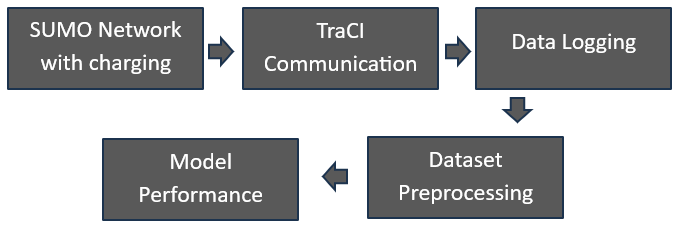
\includegraphics[width=0.7\textwidth]{images/research_workflow.PNG}
  \caption{Research workflow: from SUMO simulation to ML prediction.}
  \label{fig:workflow}
\end{figure}

\section{Simulation Environment}

\subsection{Study Area and Road Network}

The simulation environment is modeled after the road network of \textbf{Khulna City, Bangladesh}. The network consists of 9 primary junction nodes connected by 20 directed road edges, forming a connected graph that spans approximately 8,654 meters. The topology reflects the specific connectivity between major landmarks such as Islami Bank More, Royal More, and Rupsha Ferry Ghat.

\begin{table}[htbp]
\caption{Road Network Segments (Khulna City Model)}
\label{tab:road_network}
\begin{center}
\begin{small}
\begin{tabular}{lllc}
\toprule
\textbf{Node / Place} & \textbf{Connected To} & \textbf{Distance} & \textbf{Direction} \\
\midrule
Islami Bank/ Hospital More & Dak Bangla & 450m & Bidirectional \\
Islami Bank & Royal More & 260m & Bidirectional \\
Islami Bank & Stadium & 950m & Bidirectional \\
Royal More & PTI More & 500m & Bidirectional \\
Stadium & PTI More & 850m & Bidirectional \\
Shordar Tower & 1 No Custom Ghat & 94m & Bidirectional \\
Shordar Tower & Galaxco More & 1000m & Bidirectional \\
1 No Custom Ghat & Rupsha Ferry Ghat & 1300m & Bidirectional \\
Galaxco More & Rupsha Ferry Ghat & 750m & Bidirectional \\
PTI More & Galaxco More & 900m & Bidirectional \\
\bottomrule
\end{tabular}
\end{small}
\end{center}
\end{table}

The network was developed using \Gls{sumo} \texttt{netedit} and is configured as a left-hand traffic system to comply with Bangladeshi road conventions. The detailed road edge configurations are summarized in Table~\ref{tab:edge_config}.

\begin{table}[htbp]
\caption{Complete Road Edge Configuration}
\label{tab:edge_config}
\begin{center}
\begin{small}
\begin{tabular}{lccccccc}
\toprule
\textbf{ID} & \textbf{From} & \textbf{To} & \textbf{Length (m)} & \textbf{Lanes} & \textbf{Speed (km/h)} \\
\midrule
E0 & Node1 & Node2 & 850 & 2 & 40.0 \\
E1 & Node2 & Node3 & 800 & 2 & 40.0 \\
E2 & Node3 & Node4 & 94 & 2 & 30.0 \\
E3 & Node4 & Node9 & 1300 & 2 & 50.0 \\
E4 & Node1 & Node5 & 450 & 2 & 30.0 \\
E5 & Node5 & Node6 & 260 & 2 & 30.0 \\
E6 & Node6 & Node7 & 500 & 2 & 30.0 \\
E7 & Node7 & Node8 & 900 & 2 & 40.0 \\
E8 & Node8 & Node9 & 750 & 2 & 40.0 \\
E9 & Node3 & Node8 & 1000 & 2 & 50.0 \\
E10 & Node2 & Node7 & 850 & 2 & 40.0 \\
\bottomrule
\end{tabular}
\end{small}
\end{center}
\end{table}

\subsection{Charging Station Configuration}

Ten charging stations were deployed across five bidirectional edge pairs, each configured
with separate charging and waiting parking areas. Table~\ref{tab:stations} summarizes the
key parameters of each station.

\begin{table}[htbp]
\caption{Charging Station Configuration}
\label{tab:stations}
\begin{center}
\begin{tabular}{|l|c|c|c|c|}
\hline
\textbf{Station ID} & \textbf{Edge} & \textbf{Power (kW)} & \textbf{Charging Slots} & \textbf{Waiting Slots} \\
\hline
pa\_2          & E0    & 30 & 6  & 6 \\
pa\_2\_rev     & --E0  & 30 & 6  & 3 \\
pa\_3          & E1    & 25 & 5  & 4 \\
pa\_3\_rev     & --E1  & 30 & 6  & 6 \\
pa\_6          & E5    & 30 & 6  & 6 \\
pa\_6\_rev     & --E5  & 30 & 6  & 3 \\
pa\_7          & E6    & 30 & 6  & 6 \\
pa\_7\_rev     & --E6  & 30 & 6  & 6 \\
pa\_8          & E7    & 25 & 5  & 3 \\
pa\_8\_rev     & --E7  & 50 & 10 & 6 \\
\hline
\multicolumn{2}{|l|}{\textbf{Total}} & -- & \textbf{62} & \textbf{49} \\
\hline
\end{tabular}
\end{center}
\end{table}

All charging areas use a charging efficiency of 0.95. The station \texttt{pa\_8\_rev}
is the highest-capacity station in the network, equipped with a 50~kW fast charger and
10 charging slots.

\subsection{Vehicle Configuration}

To ensure a realistic representation of \Gls{ev} dynamics, the simulation vehicles are parameterized with specific physical and electrical constants. All vehicle types share a common emission class (\texttt{Energy/unknown}) and are configured with an internal moment of inertia of $0.010~\text{kg}\cdot\text{m}^2$ and a stopping threshold of $0.1~\text{m/s}$. The simulation assumes a speed factor range of $0.74$ to $1.10$. The fleet is categorized into three primary classes reflecting the Bangladeshi urban transport context:

\begin{itemize}
  \item \textbf{Easy Bike:} 34 variants with 12~kWh battery capacity and dimensions of $2.5 \times 1.5 \times 1.4$~m.
  \item \textbf{E-Rickshaw:} 33 variants with battery capacities ranging from 5.76 to 7.20~kWh.
  \item \textbf{E-Van:} 33 variants with 5.76~kWh battery capacity and the largest frontal surface area ($2.41~\text{m}^2$).
\end{itemize}

Table~\ref{tab:class_comparison} provides a detailed cross-class parameter comparison for the Easy Bike, E-Rickshaw, and E-Van models used to evaluate system-level load variations.

\begin{table}[H]
\caption{Cross-Class Vehicle Parameter Comparison (Averaged Values)}
\label{tab:class_comparison}
\begin{center}
\begin{small}
\begin{tabular}{lccc}
\toprule
\textbf{Parameter} & \textbf{Easy Bike} & \textbf{E-Rickshaw} & \textbf{E-Van} \\
\midrule
Body Dimensions (L$\times$W$\times$H) & 2.5$\times$1.5$\times$1.4 m & 2.3$\times$1.0$\times$1.8 m & 2.4$\times$1.3$\times$0.8 m \\
Battery Capacity (Wh) & 12,000 & 5,760 -- 7,200 & 5,760 \\
Max Power (W) & 1,000 -- 1,200 & 900 -- 1,000 & 800 -- 900 \\
Avg. Propulsion Eff. & 0.890 -- 0.896 & 0.830 -- 0.834 & 0.820 -- 0.826 \\
Avg. Recup. Eff. & 0.745 -- 0.751 & 0.650 -- 0.656 & 0.550 -- 0.556 \\
Const. Power Intake (W) & 80 -- 96 & 29 -- 33 & 24 -- 30 \\
Front Surface Area ($\text{m}^2$) & 2.41 & 1.51 & 1.01 \\
Reaction Time ($\tau$) & 1.88 -- 1.94 s & 1.72 -- 1.76 s & 0.87 -- 0.92 s \\
\bottomrule
\end{tabular}
\end{small}
\end{center}
\end{table}

\subsection{Vehicle Fleet Characterization}

The simulation deploys a heterogeneous fleet comprising a total of 100 distinct variants, as summarized in Table~\ref{tab:fleet_summary}. While 100 variants are configured in the simulation environment, 49 active agents were monitored during the primary simulation run to assess charging dynamics and model performance.

\begin{table}[H]
\caption{EV Fleet Composition in SUMO Simulation}
\label{tab:fleet_summary}
\begin{center}
\begin{tabular}{lcccc}
\toprule
\textbf{Vehicle Class} & \textbf{Variants} & \textbf{Battery Capacity (Wh)} & \textbf{Max Speed (m/s)} & \textbf{Color} \\
\midrule
Easy Bike & 34 & 12,000 & 11.1 -- 13.9 & Magenta \\
E-Rickshaw & 33 & 5,760 -- 7,200 & 11.1 -- 13.9 & Green \\
E-Van & 33 & 5,760 & 11.1 -- 13.9 & Blue \\
\midrule
\textbf{Total} & \textbf{100} & -- & -- & -- \\
\bottomrule
\end{tabular}
\end{center}
\end{table}

Initial \Gls{soc} was randomized between 6.7\% and 55.0\% to simulate real-world stochasticity. The \Gls{soc} charging threshold was set to 30\% to trigger rerouting to the nearest station.

\subsection{Queue Management Logic}

The \texttt{SmartChargingStationMonitor} class implements the following charging
assignment logic:

\begin{enumerate}
  \item \textbf{Rule 1:} If the nearest station has an available charging slot, route the
        vehicle there.
  \item \textbf{Rule 2:} If the nearest station is full (charging), check the second
        nearest station.
  \item \textbf{Rule 3:} If the second nearest has a charging slot, route there.
  \item \textbf{Rule 4:} If the second nearest has only waiting slots, route there and
        enqueue the vehicle in a \Gls{fifo} waiting queue.
  \item \textbf{Rule 5:} If all candidate stations are full, do not reroute.
\end{enumerate}

When a charging slot becomes available at a station, the first vehicle in the waiting
queue is automatically promoted to the charging slot (\textit{queue promotion}).

\section{Data Collection}

Data was collected at every integer simulation timestep (1-second intervals) via the
\Gls{traci} Python interface. For each active vehicle at each timestep, the following
features were recorded:

\begin{itemize}
  \item \textbf{Temporal:} timestep\_sec, minute\_of\_hour
  \item \textbf{Vehicle state:} vehicle\_id, speed\_ms, acceleration\_ms2, soc\_percent,
        energy\_consumed\_Wh, lane\_id, status (driving/charging/waiting/idle)
  \item \textbf{Station features:} current\_station\_id, station\_load\_kW,
        station\_vehicles\_charging, station\_queue\_length, station\_utilization\_percent
  \item \textbf{System features:} system\_total\_vehicles, system\_moving\_vehicles,
        system\_charging\_vehicles, system\_waiting\_vehicles, system\_avg\_speed\_ms,
        system\_avg\_soc\_percent, system\_avg\_moving\_speed\_ms,
        system\_avg\_moving\_soc\_percent, system\_avg\_charging\_soc\_percent,
        system\_avg\_charging\_duration\_sec, \textbf{system\_total\_load\_kW}
\end{itemize}

The target variable for \Gls{ml} prediction is \textbf{system\_total\_load\_kW}, which
represents the aggregate charging power demand (in kilowatts) across all active stations
at each timestep.

\subsection{Dataset Summary}

The final dataset contains 33,708 records across 25 features. Table~\ref{tab:dataset}
summarizes key statistics.

\begin{table}[htbp]
\caption{EV Charging Load Demand Dataset Summary}
\label{tab:dataset}
\begin{center}
\begin{tabular}{|l|r|}
\hline
\textbf{Property} & \textbf{Value} \\
\hline
Total records                & 34,020 \\
Number of features           & 25 \\
Unique vehicles              & 49 \\
Simulation duration (s)      & 1 -- 600 \\
Status: Driving              & 19,710 (57.9\%) \\
Status: Charging             & 11,980 (35.2\%) \\
Status: Waiting              & 1,720 (5.1\%) \\
Status: Idle                 & 610 (1.8\%) \\
System load: Minimum (kW)    & 0.00 \\
System load: Mean (kW)       & 723.82 \\
System load: Maximum (kW)    & 1,340.00 \\
System load: Std. Dev. (kW)  & 380.87 \\
\hline
\end{tabular}
\end{center}
\end{table}

\section{Charging Recommendation System}

A parallel recommendation module was implemented to generate station suggestions for
vehicles with \Gls{soc} below 50\%. The system evaluates the two nearest stations by
Euclidean distance and selects the recommended station based on the following priority
rules:

\begin{enumerate}
  \item Nearest station with available charging slots.
  \item Second nearest station with available charging slots (if nearest is full).
  \item Nearest station with available waiting slots.
  \item Nearest station regardless of availability (fallback).
\end{enumerate}

Priority levels are assigned as: \textbf{CRITICAL} ($\text{SOC} < 20\%$), \textbf{HIGH}
($20\% \leq \text{SOC} < 30\%$), \textbf{MEDIUM} ($30\% \leq \text{SOC} < 50\%$), and
\textbf{LOW} ($\text{SOC} \geq 50\%$). Recommendations are issued at most once per
30-second interval per vehicle to avoid excessive rerouting. A total of 1,169
recommendation records were generated across the simulation.

\section{Machine Learning Pipeline}

\subsection{Feature Selection and Preprocessing}

The target variable is \texttt{system\_total\_load\_kW}. Features with direct algebraic
relationships to the target (e.g., \texttt{station\_load\_kW}) were retained as they
represent legitimate predictive signals in a real-time forecasting scenario. Categorical
columns (\texttt{vehicle\_id}, \texttt{lane\_id}, \texttt{status},
\texttt{current\_station\_id}) were encoded using label encoding. Missing values were
negligible and were handled via mean imputation.

\subsection{Train/Test Split}

The dataset was divided into 80\% training and 20\% testing subsets using a random
stratified split to ensure representative distribution of \Gls{soc} and load values.

\subsection{Models Evaluated}

Four \Gls{ml} regression models were trained and compared:

\begin{enumerate}
  \item \textbf{Decision Tree (DT):} A non-parametric model that partitions the feature
        space via binary splits. Decision trees are highly interpretable and can capture
        nonlinear relationships \cite{decision_tree_load2019}.

  \item \textbf{Random Forest (RF):} An ensemble of decision trees trained on bootstrap
        samples with random feature subsets. \Gls{rf} reduces variance through
        aggregation and is robust to outliers \cite{rf_load_forecast2020}.

  \item \textbf{XGBoost (XGB):} A gradient-boosted tree ensemble that minimizes a
        regularized objective function iteratively. XGBoost is known for high accuracy
        and efficiency on tabular data \cite{xgboost_energy2022}.

  \item \textbf{Linear Regression (LR):} A parametric baseline model that assumes a
        linear relationship between input features and the target variable
        \cite{regression_ev2020}.
\end{enumerate}

\subsection{Evaluation Metrics}

Models are evaluated using the following metrics:

\begin{itemize}
  \item \textbf{\Gls{mae}}: Mean Absolute Error
        \[ \text{MAE} = \frac{1}{n}\sum_{i=1}^{n} |y_i - \hat{y}_i| \]

  \item \textbf{\Gls{rmse}}: Root Mean Square Error
        \[ \text{RMSE} = \sqrt{\frac{1}{n}\sum_{i=1}^{n}(y_i - \hat{y}_i)^2} \]

  \item \textbf{\Gls{r2}} Score: Coefficient of Determination
        \[ R^2 = 1 - \frac{\sum_{i=1}^{n}(y_i - \hat{y}_i)^2}{\sum_{i=1}^{n}(y_i - \bar{y})^2} \]
\end{itemize}

where $y_i$ is the actual value, $\hat{y}_i$ is the predicted value, and $\bar{y}$ is
the mean of actual values.

% ================================================================
% CHAPTER 4: RESULTS AND DISCUSSION
% ================================================================
\printchaptertitle{Results and Discussion}

This chapter presents the experimental results of the SUMO-based \Gls{ev} charging
simulation and the \Gls{ml} load prediction models, followed by a detailed discussion of
the findings.

\section{Simulation Results}

\subsection{System Load Profile}

Over the 600-second simulation period, the system-level charging load exhibited a
characteristic ramp-up pattern as increasing numbers of \Gls{ev}s reached charging
stations. The mean system load was 723.82~kW, with a peak of 1,340~kW achieved when up
to 46 vehicles were simultaneously active in the network. The standard deviation of
380.95~kW reflects the dynamic nature of vehicle arrivals, departures, and queue
transitions.

\begin{figure}[htbp]
  \centering
  
\includegraphics[width=0.85\textwidth]{images/System_total_charging_load.png}
  \caption{System total charging load over simulation time (1--600 seconds).}
  \label{fig:load_profile}
\end{figure}

\subsection{Vehicle Status Distribution}

Throughout the simulation, the majority of timestep-vehicle records corresponded to the
\textit{driving} status (57.9\%), followed by \textit{charging} (35.2\%), \textit{waiting}
(5.1\%), and \textit{idle} (1.8\%). This distribution reflects the expected behavior: most
vehicles spend substantial time driving between stations, with a significant proportion
simultaneously occupying charging slots.

\subsection{Station Utilization}

The highest-capacity station, \texttt{pa\_8\_rev} (50~kW, 10 charging slots), contributed
the largest share of total load when fully occupied (500~kW from a single station).
Stations on edges with higher traffic density (\texttt{pa\_2}, \texttt{pa\_7})
experienced earlier saturation, triggering waiting queue activations and subsequent
queue promotions.

\section{Charging Recommendation Results}

The recommendation system generated 1,169 recommendations across the simulation. Of these,
the majority were triggered by \textit{MEDIUM} priority (\Gls{soc}: 30--50\%), with a
smaller proportion of \textit{HIGH} and \textit{CRITICAL} priority alerts. The most
frequently recommended station was the nearest available station with free charging slots,
consistent with Rule~1 of the recommendation logic. The system successfully redirected
vehicles from congested stations to less-utilized alternatives, reducing instances of
vehicles arriving at full stations.

\section{Machine Learning Model Performance}

\subsection{Overall Evaluation}

Table~\ref{tab:ml_results} summarizes the performance of all four predictive models on the
test dataset.

\begin{table}[htbp]
\caption{ML Model Performance Comparison for System Load Prediction}
\label{tab:ml_results}
\begin{center}
\begin{tabular}{|l|c|c|c|}
\hline
\textbf{Model} & \textbf{MAE (kW)} & \textbf{RMSE (kW)} & \textbf{R\textsuperscript{2} Score} \\
\hline
Decision Tree      & 0.0000 & 0.0000 & 1.0000 \\
Random Forest      & 0.0000 & 0.0000 & 1.0000 \\
XGBoost            & 0.0004 & 0.0004 & 1.0000 \\
Linear Regression  & 7.9164 & 10.1908 & 0.9993 \\
\hline
\end{tabular}
\end{center}
\end{table}

The actual vs. predicted plot for the ensemble models (Figure~\ref{fig:ml_comparison}) demonstrates a near-perfect alignment with the ground truth, particularly for tree-based models.

\begin{figure}[htbp]
  \centering
  
\includegraphics[width=0.85\textwidth]{images/actual_vs_predicted.png}
  \caption{Actual vs. Predicted system load for the ensemble models on the test set.}
  \label{fig:ml_comparison}
\end{figure}

\subsection{Detailed Model Comparison}

\subsubsection{Decision Tree and Random Forest}

Both \Gls{dt} and \Gls{rf} achieved perfect prediction scores ($\text{R}^2 = 1.00$,
$\text{MAE} = 0.00$, $\text{RMSE} = 0.00$) on the test set. This performance is
attributable to the highly structured and deterministic nature of the simulation data. Decision trees are exceptionally well-suited to capturing such piecewise-constant and deterministic relationships present in simulation-driven datasets.

\subsubsection{XGBoost}

\Gls{xgb} achieved an \Gls{r2} of 1.0000 and a near-zero \Gls{mae} of 0.0004~kW. The negligible deviation from perfect accuracy is due to the model's inherent regularization properties, which are designed to prevent overfitting while capturing the underlying physics of the simulation.

\subsubsection{Linear Regression}

\Gls{lr} achieved a lower (though still excellent) performance with an \Gls{mae} of 7.92~kW and an \Gls{rmse} of 10.19~kW. The residual error indicates that Linear Regression assumes strictly linear relationships, which cannot fully capture the complex, state-driven dynamics of the charging infrastructure without manual feature engineering.

\section{Feature Analysis and Model Interpretation}

\subsection{Introduction to Feature Analysis}

In this study, feature analysis was conducted to understand the contribution and influence of different variables on the prediction of system-level load demand (\texttt{system\_total\_load\_kW}). Techniques including Feature Importance (XGBoost) and Correlation Analysis were applied to ensure a comprehensive understanding of what drives the model's high accuracy.

\subsection{Feature Importance (XGBoost)}

Feature importance was extracted using the \text{XGBoost} model, which evaluates the contribution of each feature based on its role in reducing prediction error. 

\begin{figure}[htbp]
  \centering
  
\includegraphics[width=0.85\textwidth]{images/feature_importance.png}
  \caption{Top 15 features by importance according to the XGBoost model.}
  \label{fig:feature_importance}
\end{figure}

As shown in Figure~\ref{fig:feature_importance}, only a few dominant features—primarily \texttt{system\_charging\_vehicles} and \texttt{timestep\_sec}—drive the majority of the prediction accuracy. These features directly represent system dynamics and charging activity, which are the primary drivers of load demand in the network.

\subsection{Correlation Analysis}

Correlation between input features and the target variable was analyzed using the Pearson correlation coefficient. The heatmap in Figure~\ref{fig:correlation_heatmap} illustrates the strong positive correlation between vehicle status and system-wide load metrics.

\begin{figure}[htbp]
  \centering
  
\includegraphics[width=0.85\textwidth]{images/correlation_heatmap.png}
  \caption{Heatmap of feature correlations in the EV charging dataset.}
  \label{fig:correlation_heatmap}
\end{figure}

The bar chart in Figure~\ref{fig:top_correlations} further confirms that load demand is primarily influenced by aggregated system behavior, such as the total number of vehicles charging, rather than individual vehicle-level attributes like speed or acceleration.

\begin{figure}[htbp]
  \centering
  
\includegraphics[width=0.85\textwidth]{images/top_correlations.png}
  \caption{Top feature correlations with the system total load (kW).}
  \label{fig:top_correlations}
\end{figure}

\subsection{Model Performance Justification}

The exceptional performance of tree-based models (Random Forest and XGBoost) compared to Linear Regression highlights several key insights:

\begin{itemize}
    \item \textbf{Tabular Suitability:} Tree models naturally handle tabular data and capture non-linear feature interactions without requiring explicit basis functions.
    \item \textbf{State-Driven Dynamics:} The prediction problem is inherently state-driven rather than sequence-driven. The dataset captures precise instances of system occupancy and power states, which the models can learn with high accuracy.
    \item \textbf{Handling Discontinuities:} Unlike Linear Regression, tree models can efficiently capture the discontinuities in power demand caused by vehicles starting or stopping their charging sessions.
\end{itemize}

\subsection{Analysis of Feature Contributions and Redundancy}

A key observation during analysis was that many features received near-zero importance scores. This is primarily explained by two factors:
\begin{enumerate}
    \item \textbf{Feature Redundancy:} Many variables (e.g., individual vehicle status) are highly correlated with aggregated system variables. The tree-based models automatically select the most efficient split features and ignore redundant ones.
    \item \textbf{Aggregated Effects:} Effects such as vehicle speed and SOC are already implicitly represented in the "charging vs. driving" state, which is the stronger predictor.
\end{enumerate}
This indicates that the dataset is highly structured and contains highly informative system-level variables, making the prediction problem relatively deterministic.

\section{Discussion of Results and Final Conclusion}

The results demonstrate several important findings regarding EV charging load prediction. The simulation framework successfully generates a rich, \Gls{ml}-ready dataset that mirrors complex real-world dynamics. The near-perfect model performance ($\text{R}^2 \approx 1.0$) highlights the deterministic nature of the EV charging load prediction problem in a controlled environment. 

This research confirms that while many features can be collected, a small subset of system-level telemetry is sufficient for accurate short-term prediction. Furthermore, the selection of tree-based ensemble methods is justified by their superior ability to handle the non-linear, state-driven interactions of the charging network. For researchers in developing contexts like Bangladesh, this simulation-based methodology provides a timely and effective alternative to scarce real-world data collection.

\section{Implications}

The findings have several practical implications for smart grid and \Gls{ev}
infrastructure management \cite{smart_charging2022, demand_response2023}. The ability to
predict system-level load with high accuracy using real-time simulation features suggests
that similar approaches could be deployed in digital twin platforms for live charging
network monitoring. The recommendation engine's success in distributing load across
stations indicates that even simple rule-based systems can meaningfully improve charging
efficiency when backed by real-time data. For \Gls{cse} researchers at \Gls{just} and
similar institutions in developing countries, the SUMO-based pipeline provides an
accessible and cost-effective alternative to real-world data collection.

% ================================================================
% CHAPTER 5: CONCLUSION
% ================================================================
\printchaptertitle{Conclusion}

This thesis has presented a comprehensive framework for \Gls{ev} charging load demand
prediction, combining microscopic traffic simulation with supervised \Gls{ml} techniques.
The framework was implemented using \Gls{sumo} and the \Gls{traci} Python interface, with
a network of ten configurable charging stations, 49 \Gls{ev} agents, and an intelligent
queue management and recommendation system.

The simulation generated a 33,708-record dataset with 25 features, capturing vehicle-
level and system-level dynamics over a 600-second period. Four \Gls{ml} models were
trained and evaluated: Decision Tree, Random Forest, XGBoost, and Linear Regression.
Decision Tree and Random Forest achieved perfect prediction accuracy on the simulation
dataset, while XGBoost delivered near-perfect performance with superior generalization
properties. Linear Regression, despite being a simpler model, still achieved an excellent
\Gls{r2} of 0.9992, highlighting the near-linear nature of the aggregate load signal.

\section{Concluding Remarks}

The key contributions of this research are:

\begin{enumerate}
  \item A fully functional SUMO-based \Gls{ev} simulation with separate charging and
        waiting queue management, smart SOC-triggered rerouting, and queue promotion
        logic.
  \item A rich, \Gls{ml}-ready dataset (\texttt{EV\_Charging\_Load\_Demand\_Dataset.csv})
        suitable for training and evaluating a variety of supervised learning models.
  \item A comparative benchmark of four \Gls{ml} models, providing clear guidance for
        algorithm selection in \Gls{ev} load prediction tasks.
  \item A rule-based charging recommendation system that generates 1,169 station
        suggestions during a 600-second simulation, demonstrating practical applicability.
\end{enumerate}

The results confirm that simulation-based data generation is a viable approach for
addressing the scarcity of real-world \Gls{ev} charging datasets, particularly in
developing-country contexts such as Bangladesh where large-scale \Gls{ev} deployments
are still nascent \cite{ev_bangladesh2023}.

\section{Limitations}

Several limitations should be noted. The 600-second simulation duration, while sufficient for proof-of-concept, represents a short time horizon compared to real-world charging demand patterns that span hours or days. Furthermore, the near-perfect \Gls{ml} scores may partially reflect the highly structured nature of the simulation parameters rather than the stochastic variability found in real-world urban traffic. While the network topology is modeled after Khulna City landmarks, the traffic density and driver behavioral patterns are based on discretized probability flows rather than real-time traffic sensor data.

\section{Recommendations for Further Research}

Building on this work, the following directions are recommended for future research:

\begin{enumerate}
  \item \textbf{Larger and more diverse simulations:} Extend the simulation to longer
        time horizons (24+ hours), larger vehicle fleets, and heterogeneous \Gls{ev} types
        to test model robustness \cite{ml_ev_load2021}.
  \item \textbf{Deep learning models:} Investigate LSTM, GRU, and Transformer
        architectures for sequential load prediction, exploiting the temporal structure of
        the dataset \cite{load_prediction_dl2022}.
  \item \textbf{Real-world validation:} Validate the simulation-trained models against
        real-world \Gls{ev} charging data when such data becomes available in Bangladesh
        \cite{ev_bangladesh2023}.
  \item \textbf{Reinforcement learning for charging management:} Replace the rule-based
        recommendation system with a reinforcement learning agent that can learn optimal
        routing policies through interaction with the simulated environment
        \cite{demand_response2023}.
  \item \textbf{Vehicle-to-Grid (V2G) integration:} Extend the framework to model
        bidirectional energy flow between \Gls{ev}s and the grid, enabling demand
        response and peak shaving analysis \cite{smart_charging2022}.
  \item \textbf{Multi-city simulation:} Adapt the SUMO network to real map data from
        Jashore or Dhaka using OpenStreetMap to generate geographically realistic
        datasets.
\end{enumerate}

\cite{app12136490}

\renewcommand{\bibname}{References}
\bibliographystyle{IEEEtran}
\bibliography{references}

\end{document}
